Based on the discussed practical applications and novel visualization approaches, one can see that there is no such tool combining thematic maps with animations when changing visual appearance. The advantages and disadvantages of all aspects have been broached and discussed. This thesis will furthermore discuss and show a novel approach based on the concept of unit visualizations combined with classical thematic maps and animations when changing visual appearance. However, there are multiple possible solutions. This section will discuss some solutions with the requirement of building an an interactive web application. The solutions should yield answers to the question of which tasks can be supported by particle aggregation in thematic maps and how can the aggregation be realized.

In order to realize a practical solution for the given question, it is assumed that a dataset including heterogeneous data and some kind of geospatial data is given.

According to the mantra of \citeauthor{Shneiderman1996}, the application should start by giving an overview of the dataset. With the main concept in mind, there are two possible solutions:
\begin{enumerate}

\ditem{Unit-based grid} \hfill \\
SandDance features an approach of showing a grid as visualization, where all data items are represented as some kind of shape. Figure \ref{fig:sanddance-grid} on page \pageref{fig:sanddance-grid} shows the implementation of a unit-based grid.

\begin{figure}[!htb]
\centering
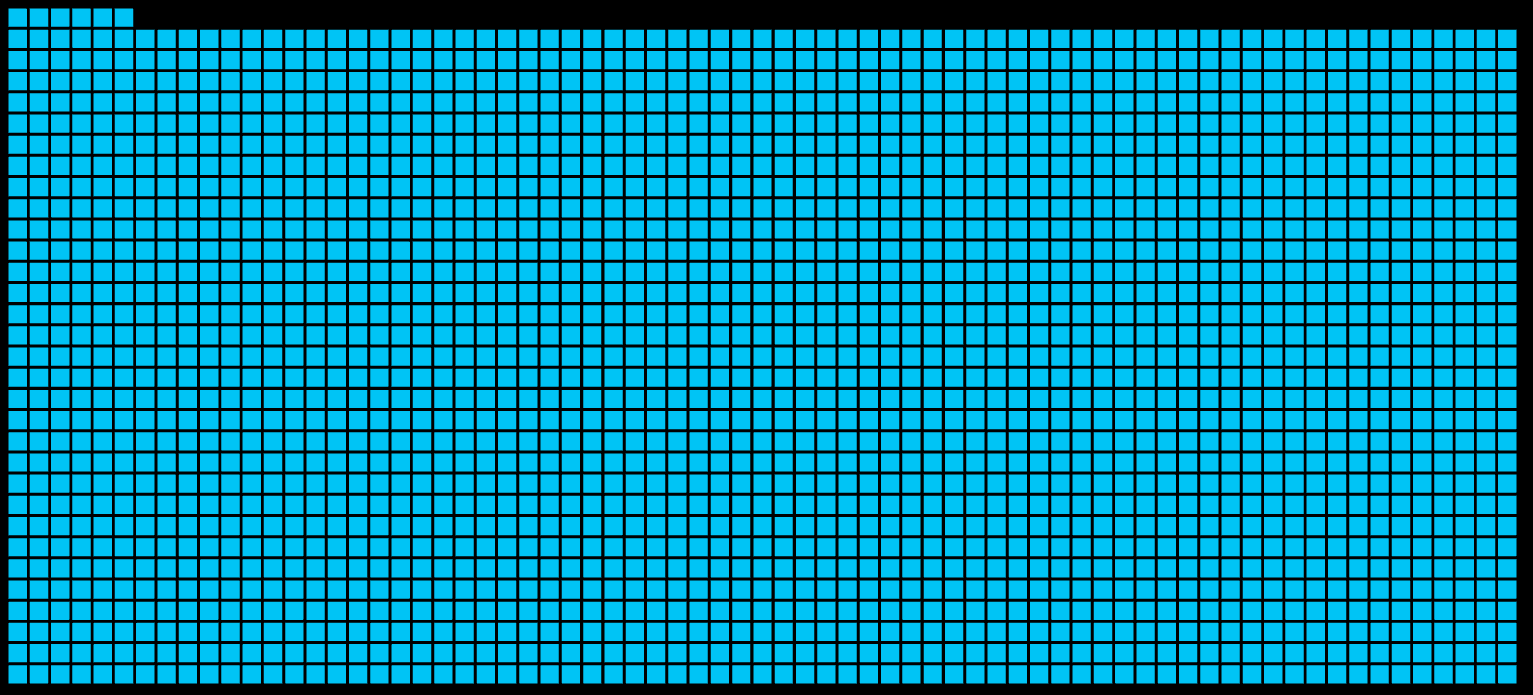
\includegraphics[height=5cm]{images/methods/related/sanddance-grid.png}
\caption[
    Unit-based grid in SandDance.
]{Unit-based grid in SandDance}
\label{fig:sanddance-grid}
\end{figure}

\ditem{Dot map} \hfill \\
Chapter \ref{s:dot} on page \pageref{s:dot} discusses the concept of dot maps in detail. This kind of thematic map can be used in combination with a one-to-one relation ship and show every item in the dataset as a single dot on the map giving an overview of the whole dataset including its geographical distribution.

\ditem{Particle attractor} \hfill \\
Figure \ref{fig:particle-attractor} on page \pageref{fig:particle-attractor} sketches the concept of showing all data items around a particle attractor.

\begin{figure}[!htb]
\centering
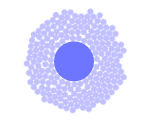
\includegraphics[height=5cm]{images/methods/related/particle-attractor.png}
\caption[
    Particle attractor sketch.
]{Particle attractor sketch}
\label{fig:particle-attractor}
\end{figure}

\end{enumerate}

The next step after having an overview is to decide which tasks to try out in order to test particle aggregation. One big part of this thesis already dicsusses thematic cartography in detail and thus the decision of using different types of thematic maps, which are all based on some kind of aggregation, is reasonable. Therefore trying animated particle aggregation in combination with proportional symbol maps, choropleth maps and cartograms will be a main part of the practical approach. However, there are multiple ways in changing visual appearance from an overview of the data to some kind of thematic map.

\begin{enumerate}

\ditem{In-place transition} \hfill \\
Changing from one kind of a thematic map to another one with in-place transition denotes the concept of creating the upcoming visualization. Starting with an overview grid and having a dot map as an upcoming visualization would move all particles in the same canvas to their geographical position. Having a map in the background when changing from an abstract grid to a thematic map could support the comprehensibility.
If the user determines to change the visual appearance to some other kind of thematic map, the particles would need to move according to the characteristics of the upcoming visualization. Without consideration of using other visual channels except motion, in-place transitions have multiple advantages:
\begin{itemize}
\item Semantic constancy
\item Amount of particles stays the same throughout the application (this becomes more clear when reading non in-place transitions)
\end{itemize}

\ditem{Non in-place transitions} \hfill \\
Animating the transition from one thematic map to another can also be done with an adaption of the multiple views concept. \citeauthor{Javed2012} present different visualization compositions which can be adopted for animated transitions aswell \iacite{Javed2012}:
\begin{itemize}
\item \textbf{Juxtaposition:} placing visualizations side-by-side in one view
\item \textbf{Superimposition:} overlaying two visualizations in one view
\item \textbf{Overloading:} utilizing the space of one visualization
\item \textbf{Nesting:} nesting the contents of one visualization inside another one
\end{itemize}

All of the mentioned compositions can be accomplished in two different ways. Either each particle updates its position according to the upcoming visualization, or each particle is cloned and the clone updates its position accordingly. The latter method has the major drawback of scaling poorly, because a datasize with $n$ items would need $2*n$ particles when changing the visual appearance.
\end{enumerate}

Both transition types perhaps share the same advantage: using some kind of animated transition between two different visual appearances for the same data could support the readability of the visualization. Howsoever the particles move, it could help to understand how the visualization is created and therefore could support knowledge construction.
However, starting with a particle attractor as an overview, it is also possible to use this attractor to animate the creation and transizion of visualizations. Creating marks on a visual representation could be done in two ways:

\begin{enumerate}
\item Each particle tags its spot on the map by leaving an abstract, static mark
\item Each particle moves to its spot on the map and stays
\end{enumerate}

The first method would yield animated creations, with a very basic approach when changing the visual appearance. All particles would draw upcoming visualizations every time, without considering some kind of transition from the first to the second one. The second approach can be used to initially draw the first thematic map when no other visualization is given. Changing the visual appearance if a thematic map is already shown, the mentioned transition methods can be used.

%https://imgur.com/eRDNsj3
Considering the transition from a dot map to any other type of thematic map, the aggregation needs to be animated. Figure \ref{} on page \pageref{} shows nine different ways of how particles are able to fit in or interact with a perimeter of a given abstract shape. This heavily influences the movement of particles and the readability of the map. Aggregation can not only be done by moving the particle to their new aggregated shape. It could also be accomplished by using the concept of visual sedimentation, but it would also inherit its major weakness of not showing a static when using static data. When using the concept of SandDance of building aggregated shapes with units, a map will suffer from overplotting in high density region, thus leading to visual clutter. Therefore most of the shown unit design strategies will be unusable in combination with certain thematic maps, e.g. proportional symbol maps.

\begin{table}[!htp]
    \begin{tabular}{M{22mm}||M{22mm} M{22mm} M{22mm} M{22mm} M{22mm}}

    ~                       & Overview & Dot Map & Proportional Symbol Map & Choropleth Map & Cartogram \\[4ex] \hline \hline

    Overview                & ~        & ~       & ~                       & ~              & ~         \\[4ex]

    Dot Map                 & ~        & ~       & ~                       & ~              & ~         \\[4ex]

    Proportional Symbol Map & ~        & ~       & ~                       & ~              & ~         \\[4ex]

    Choropleth Map          & ~        & ~       & ~                       & ~              & ~         \\[4ex]

    Cartogram               & ~        & ~       & ~                       & ~              & ~         \\[4ex]
    \end{tabular}
    \caption {Table Caption}
\end{table}
